\documentclass[a4paper,notumble]{leaflet}
\usepackage[T1]{fontenc}
\usepackage[utf8]{inputenc}
\usepackage{lmodern}
\usepackage{graphicx}

% PDF properties and links
\usepackage{hyperref}
\hypersetup{
  pdfauthor   = {Sébastien Wilmet},
  pdftitle    = {GNOME Brochure},
  pdfcreator  = {Texlive},
  pdfproducer = {Texlive},
  colorlinks  = false,
  pdfborder   = 0 0 0
}

\title{The GLib/GTK+ Development Platform}
\date{}
\author{}

\begin{document}

\maketitle
\thispagestyle{empty}

GTK+, or the GIMP ToolKit, is a multi-platform toolkit for creating graphical user interfaces. Offering a complete set of widgets, GTK+ is suitable for projects ranging from small one-off tools to complete application suites.

GTK+ is written in C but has been designed from the ground up to support a wide range of languages, not only C/C++. Using GTK+ from languages such as Python and JavaScript (especially in combination with the Glade GUI builder) provides an effective method of application development.

GTK+ is free software and part of the GNU Project. However, the licensing terms for GTK+, the GNU LGPL, allow it to be used by all developers, including those developing proprietary software, without any license fees or royalties.

GTK+ has been created in 1996 for the GIMP --- the GNU Image Manipulation Program --- but has quickly become a general-purpose library used by a large number of applications including the GNU project's GNOME desktop.

\begin{center}
  
\includegraphics[width=3cm]{images/gtk-logo.pdf}
  \hspace{1cm}
  
\includegraphics[width=2cm]{images/gnome-logo.pdf}
\end{center}

\pagebreak

\section{Architecture Overview}

Over time GTK+ has been built up to be based on other libraries, also developed by the GTK+ team:
\begin{itemize}
  \item \textbf{GLib}, a low-level core library that forms the basis of GTK+. It provides data structure handling for C, portability wrappers and interfaces for such run-time functionality as an event loop, threads, dynamic loading, an object system (GObject) and high-level input/output APIs (GIO).

  \item \textbf{Pango}, a library for layout and rendering of text with an emphasis on internationalization. It forms the core of text and font handling for GTK+.

  \item \textbf{Cairo}, a library for 2D graphics with support for multiple output devices (including the X Window System, Win32) while producing a consistent output on all media while taking advantage of display hardware acceleration when available.

  \item \textbf{ATK}, a library for a set of interfaces providing accessibility. By supporting the ATK interfaces, an application or toolkit can be used with tools such as screen readers, magnifiers, and alternative input devices.

  \item \textbf{GDK}, or the GIMP Drawing Kit, is the abstraction layer that allows GTK+ to support multiple windowing systems. GDK provides backends for X11, Windows, Mac OS X, Wayland, Mir, and a web browser.
\end{itemize}

\vspace{1cm}
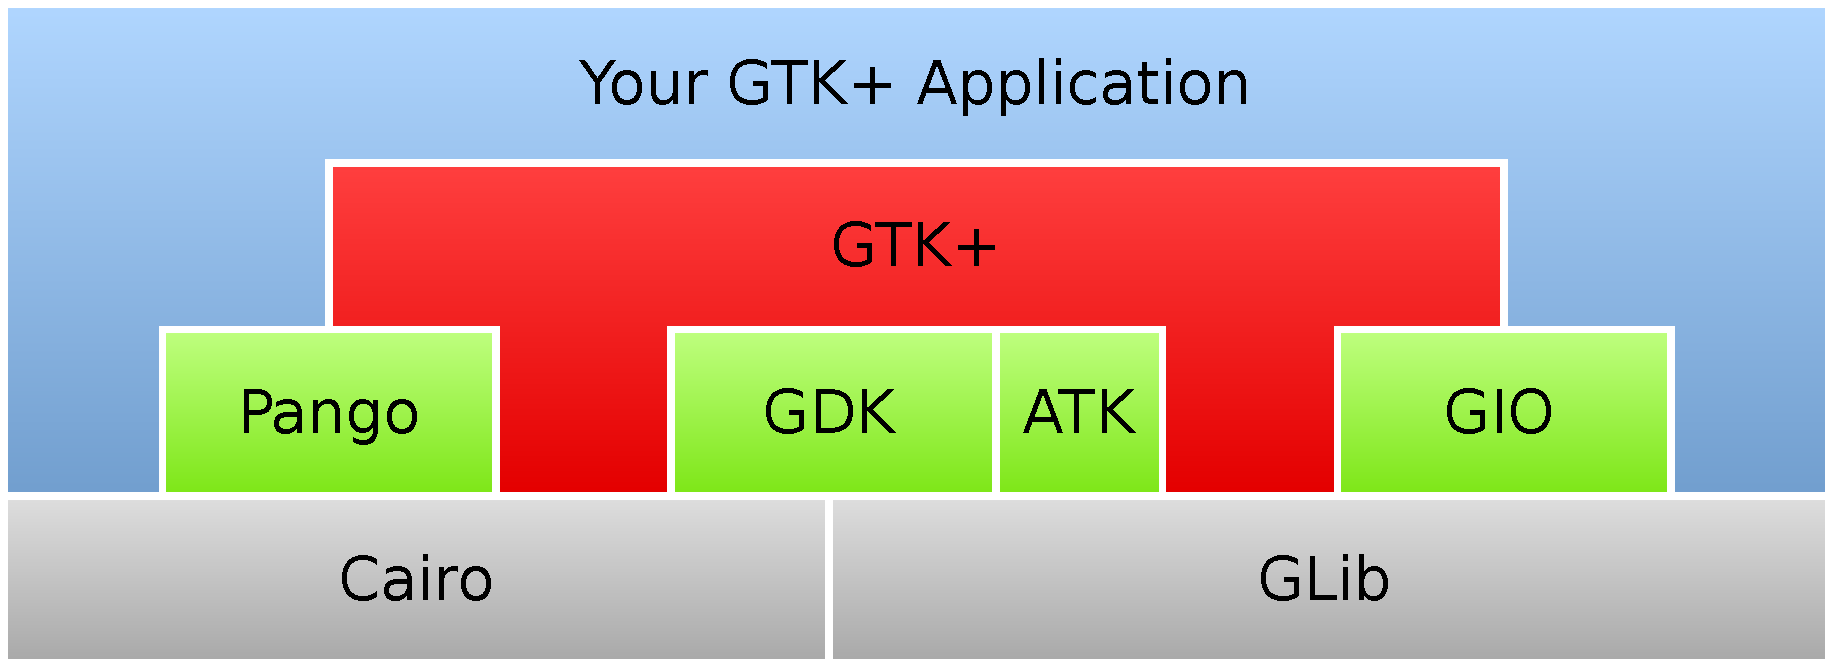
\includegraphics[width=\textwidth]{images/architecture.pdf}

\pagebreak
\section{GLib -- the Core Library}

Firstly, GLib provides common data structures:
\begin{itemize}
  \item Single and doubly linked lists.
  \item Hash tables.
  \item Balanced binary trees.
  \item N-ary trees: trees of data with any number of branches.
  \item Strings with text buffers which grow automatically as text is added.
  \item Arrays of arbitrary elements which grow automatically as elements are added.
  \item \texttt{GVariant}, a generic data type that stores a value along with information about the type of that value.
  \item And a few other data structures.
\end{itemize}

\bigskip
GLib contains also lots of utilities:
\begin{itemize}
  \item String and Unicode manipulation.
  \item Date and time functions.
  \item A command-line option parser.
  \item Perl-compatible regular expressions.
  \item An XML parser.
  \item A unit-test framework.
  \item And many other utilities.
\end{itemize}

\bigskip
Last, but not least, GLib provides some core event-driven programming features, with a \textit{main event loop}, support for threads and asynchronous communication between threads. An event loop listens some sources of events, that can come from file descriptors (plain files, pipes or sockets), timeouts, or other custom sources. A priority is associated with each source of events. When an event arrives, the event loop dispatches it to the application. The event can then be taken into account, either in the same thread or another thread.

Event-driven programming is not only useful for graphical user interfaces (with user events such as key presses and mouse clicks), but also for daemons that respond to hardware changes (a USB stick inserted, a second monitor connected, a printer low on paper), or software that listen to network connections or messages from other processes, and so on.

\section{GObject -- an Object System}

\section{GIO -- Input/Output on Steroids}

\section{The GTK+ Widget Toolkit}

\end{document}
